\chapter{Methodology: CopeOpi Vectors}
\section{From CopeOpi Scores to Augmented CopeOpi Scores}
\subsection{CopeOpi Scores}
\par CopeOpi scores\cite{ku2007score} are numeric sentiment scores of Chinese characters and Chinese words, which can be used to detect the sentiment polarities and measure the strength of sentiment polarities. The basic idea is that the meaning of a Chinese word is the function of its composing characters, so the sentiment of a Chinese word can also be determined from the sentiments of its composing characters.
\par They assume that Chinese characters in a Chinese positive opinion word tend to be positive, and Chinese characters in a Chinese negative opinion word tend to be negative. They adopt a Chinese sentiment dictionary, the NTU sentiment dictionary (NTUSD)\cite{ku2007ntusd}, as Chinese opinion seed words, and take the frequency of each Chinese character in these Chinese opinion seed words as clues to discover latent sentiments.
\par Once the CopeOpi scores of Chinese characters are available, the CopeOpi score of a Chinese word can be determined from the CopeOpi scores of its composing characters by applying a scoring function according to its morphological type\footnote{In linguistics, morphology is the study of the structure of words:   how words are formed, and their relationship to each other in a language.}, or simply taking the average\cite{ku2009morph}.
\input{chapters/ch3/figure/freqmat31.tex}
\begin{scheme}{CopeOpi Scores}{}
Given two corpora of labeled Chinese opinion words $\mathbb{W}_p$ and $\mathbb{W}_n$,
and the corresponding sentiment polarities $positive$ and $negative$.
\begin{itemize}
\item $\mathbb{W}_p = \{ w \where \text{$w$ is a Chinese opinion word labeled as $positive$} \}$
	\begin{itemize}
	\item the vocabulary $\mathbb{V}_p$ is a set of unique Chinese characters in $\mathbb{W}_p$
	\end{itemize}
\item $\mathbb{W}_n = \{ w \where \text{$w$ is a Chinese opinion word labeled as $negative$} \}$
	\begin{itemize}
	\item the vocabulary $\mathbb{V}_n$ is a set of unique Chinese characters in $\mathbb{W}_n$
	\end{itemize}
\end{itemize}
For each Chinese character $c_i \in \mathbb{V}_p \cup \mathbb{V}_n$,
we can compute its CopeOpi score $\mathcal{COP}_{c_i}$.
\begin{equation*}
\begin{gathered}
	\mathcal{P}_{c_i} = \dfrac{
		fp_{c_i} \divby \sum_{c \in \mathbb{V}_p} fp_c
	}{
		fp_{c_i} \divby \sum_{c \in \mathbb{V}_p} fp_c +
		fn_{c_i} \divby \sum_{c \in \mathbb{V}_n} fn_c
	}
\\[\eqlineskip]
	\mathcal{N}_{c_i} = \dfrac{
		fn_{c_i} \divby \sum_{c \in \mathbb{V}_n} fn_c
	}{
		fp_{c_i} \divby \sum_{c \in \mathbb{V}_p} fp_c +
		fn_{c_i} \divby \sum_{c \in \mathbb{V}_n} fn_c
	}
\\[\eqlineskip]
	\mathcal{COP}_{c_i} = \mathcal{P}_{c_i} - \mathcal{N}_{c_i}
\end{gathered}
\end{equation*}
where $\mathcal{P}_{c_i}$ and $\mathcal{N}_{c_i}$ are the normalized probabilities of
Chinese character $c_i$ being positive and being negative;
$fp_{c_i}$ and $fn_{c_i}$ are the frequencies of 
Chinese character $c_i$ in corpus $\mathbb{W}_p$ and in corpus $\mathbb{W}_n$;
the CopeOpi score $\mathcal{COP}_{c_i}$ of
Chinese character $c_i$ is defined as the difference of the two opposite normalized probabilities, ranged from
$+1$(being positive) to $-1$(being negative).
\tcbline
For each Chinese word $w_j=c_1c_2 \cdots c_l$, we can compute its CopeOpi score $\mathcal{COP}_{w_j}$.
\begin{equation*}
\mathcal{COP}_{w_j=c_1c_2\cdots c_l} =
\begin{cases}
	S_m(c_1c_2 \cdots c_l)
	& \text{if the morphological type of $w_j$ is $m$}
\\
	\dfrac{1}{l} \sum_{k=1}^l \mathcal{COP}_{c_k}
	& \text{otherwise}
\end{cases}
\end{equation*}
where $S_m$ is the scoring function of morphological type $m$.
\end{scheme}
One application of CopeOpi scores is augmented NTU sentiment dictionary (ANTUSD)\cite{wang2006antusd}, a collection of sentiment statistics of Chinese words in several sentiment annotation works. For each Chinese  word in the dictionary, the number of positive annotations, neutral annotations, negative annotations, non-opinionated annotations and not-a-word annotations are recorded, and the CopeOpi score is also provided.
\subsection{Augmented CopeOpi Scores}
\par The structure of the frequency matrix of CopeOpi scores relates to its potential applications. In the frequency matrix of CopeOpi scores, the basic units are Chinese characters and the contexts are corpora of labeled Chinese opinion words, so CopeOpi scores find their applications in Chinese sentiment analysis.
\par However, since the core of CopeOpi scores is a bag-of-units method which is generally adopted in nature language processing, we think it is possible to augment their usefulness and widen their range of applications.
\par Here we propose a new computation scheme for augmented CopeOpi scores. We transform CopeOpi scores from sentiment scores to class-tendency scores by mapping the sentiment polarities in sentiment analysis, i.e., positive or negative, to the set membership in binary classification, i.e., being in a class or not. We extend the premises and assume that words in documents of some classes tend to be in those classes. We modify the structure of the frequency matrix and
\begin{itemize}
\item change the basic units from Chinese characters to words.
\item change the contexts from corpora of Chinese opinion words to corpora of binary annotated documents.
\end{itemize}
\begin{figure}[t]
\small
\centering
\begin{tikzpicture}
	\draw[step=1cm, opacity=0] (-7,0) grid (9,0);
	\fill[black!5!white] (0,0) rectangle (2,2);
	\draw[step=1cm, double] (0,1) grid (2,2);
	\draw[step=1cm, double] (0,0) -- (0,1);
	\draw[step=1cm, double] (1,0) -- (1,1);
	\draw[step=1cm, double] (2,0) -- (2,1);
	\draw[step=1cm, dashed] (0,0) -- (2,0);
	\node (p1) at (-0.5,1.5) {$\rightarrow$};
	\node[left=-0.15cm of p1] {word $w_i$};
	\node at (1.0,3.6) {corpus of labeled documents};
	\node at (0.5,2.5) {$\downarrow$};
	\node at (1.5,2.5) {$\downarrow$};
	\node at (0.5,3) {$\mathbb{D}_p$};
	\node at (1.5,3) {$\mathbb{D}_n$};
	\node at (0.5,1.5) {$fp_{w_i}$};
	\node at (1.5,1.5) {$fn_{w_i}$};
	\node at (0.5,0.6) {$\vdots$};
	\node at (1.5,0.6) {$\vdots$};
\end{tikzpicture}
\caption[The frequency matrix of augmented CopeOpi scores]{The frequency matrix of augmented CopeOpi scores.\\
In the frequency matrix of augmented CopeOpi scores,
each row represents a unique word $w_i$ and
the two columns represent two corpora of labeled documents $\mathbb{D}_p$ and $\mathbb{D}_n$.
The elements $fp_{w_i}$ and $fn_{w_i}$ are the frequencies of word $w_i$ 
in corpus $\mathbb{D}_p$ and in corpus $\mathbb{D}_n$.}
\end{figure}
\begin{scheme}{Augmented CopeOpi Scores}{}
Given two corpora of labeled documents $\mathbb{D}_p$ and $\mathbb{D}_n$,
and the corresponding classes $p$ and $not\text{-}p$.
\begin{itemize}
\item $\mathbb{D}_p = \{ \langle d,c \rangle \where \text{$d$ is a document labeled as class $c=p$} \}$
	\begin{itemize}
	\item the vocabulary $\mathbb{V}_p$ is a set of unique words in $\mathbb{D}_p$
	\end{itemize}
\item $\mathbb{D}_n = \{ \langle d,c \rangle \where \text{$d$ is a document labeled as class $c=not\text{-}p$} \}$
	\begin{itemize}
	\item the vocabulary $\mathbb{V}_n$ is a set of unique words in $\mathbb{D}_n$
	\end{itemize}
\end{itemize}
For each word $w_i \in \mathbb{V}_p \cup \mathbb{V}_n$,
we can compute its CopeOpi score $\mathcal{COP}_{w_i}$.
\begin{equation*}
\begin{gathered}
	\mathcal{P}_{w_i} = \dfrac{
		fp_{w_i} \divby \sum_{w \in \mathbb{V}_p} fp_w
	}{
		fp_{w_i} \divby \sum_{w \in \mathbb{V}_p} fp_w +
		fn_{w_i} \divby \sum_{w \in \mathbb{V}_n} fn_w
	}
\\[\eqlineskip]
	\mathcal{N}_{w_i} = \dfrac{
		fn_{w_i} \divby \sum_{w \in \mathbb{V}_n} fn_w
	}{
		fp_{w_i} \divby \sum_{w \in \mathbb{V}_p} fp_w +
		fn_{w_i} \divby \sum_{w \in \mathbb{V}_n} fn_w
	}
\\[\eqlineskip]
	\mathcal{COP}_{w_i} = \mathcal{P}_{w_i} - \mathcal{N}_{w_i}
\end{gathered}
\end{equation*}
where $\mathcal{P}_{w_i}$ and $\mathcal{N}_{w_i}$ are the normalized probabilities of
word $w_i$ being in class $p$ and being in class $not\text{-}p$;
$fp_{w_i}$ and $fn_{w_i}$ are the frequencies of 
word $w_i$ in corpus $\mathbb{D}_p$ and in corpus $\mathbb{D}_n$;
the CopeOpi score $\mathcal{COP}_{w_i}$ of
word $w_i$ is defined as the difference of the two opposite normalized probabilities, ranged from
$+1$(being in class $p$) to $-1$(being in class $not\text{-}p$).
\end{scheme}
\partopic{Confidence in Augmented CopeOpi Scores}
\par According to Zipf's law, given some corpora of natural language, the frequency of a word is inversely proportional to its rank in the frequency table\cite{manning1999nlp}. The most frequent word occurs approximately twice as often as the second one, three times as often as the third one, etc. There are a few words that are very common and a lot of words that are very rare. Considering the later cases, we shall have less confidence in the augmented CopeOpi scores of rare words due to the lack of sufficient statistics, and besides, they are easily biased and overestimated since the occurrences of a rare word might be all in one class and absent in the other.
\par To reduce the effects of imprecise augmented CopeOpi scores of rare words, we can impose confidence values to penalize these values. We regard words whose maximal class frequency less than the average class frequency of all words as rare words, and smooth their augmented CopeOpi scores by multiplying their confidence values which is defined as a logistic function\footnote{The mentioned scheme of confidence values is merely the one we use in our experiments but not a standard scheme. You can design one for your applications.}.
\begin{equation*}
\begin{gathered}
	fc^{\max}_{w_i} = \max({fc_1}_{w_i},{fc_2}_{w_i},\dots,{fc_n}_{w_i})
\\[\eqlineskip]
	fc_{\avg} = \dfrac {
		\sum_{j=1}^m \sum_{k=1}^n {fc_k}_{w_j}
	}{
		m \times n
	}
\\[\eqlineskip]
	\mathcal{CF}_{w_i} =
	\begin{cases}
		1
		&\text{if $fc^{\max}_{w_i} \geq fc_{\avg}$}
	\\
		\dfrac{1}{1 + 3 \exp(-4(\frac{fc^{\max}_{w_i}}{fc_{\avg}}))}
		&\text{otherwise}
	\end{cases}
\\[\eqlineskip]
	\mathcal{CF}\text{-}\mathcal{COP}_{w_i} = \mathcal{CF}_{w_i} \times \mathcal{COP}_{w_i}
\end{gathered}
\end{equation*}
where ${fc_k}_{w_i}$ is the frequency of word $w_i$ in class $k$;
$fc^{\max}_{w_i}$ and $fc_{\avg}$ are the maximal class frequency of word $w_i$ and the average class frequency of all words;
$n$ and $m$ are the number of classes and the number unique words in corpora;
the confidence value $\mathcal{CF}_{w_i}$ of word $w_i$ is defined as a piece-wise function which behaves differently based on the maximal class frequency $fc^{\max}_{w_i}$ of word $w_i$.
\begin{figure}[t]
\begin{minipage}{0.5\textwidth}
	\centering
	\includegraphics[height=6cm]{chapters/ch3/figure/conf.png}
	\caption{The logistic function of $\mathcal{CF}$}
\end{minipage}
\begin{minipage}{0.5\textwidth}
	\centering
	\includegraphics[height=6cm]{chapters/ch3/figure/conf_ex.png}
	\caption{Distributions of $\mathcal{COP}$ and $\mathcal{CF}\text{-}\mathcal{COP}$}
\end{minipage}
\end{figure}

\section{From Augmented CopeOpi Scores to CopeOpi Vectors}
\subsection{CopeOpi Vectors}
\par CopeOpi scores now become augmented CopeOpi scores, class-tendency scores which can be used in languages other than Chinese since we change the basic units from Chinese characters to words, and be applied to binary text classification other than sentiment analysis since we change the contexts from corpora of Chinese opinion words to corpora of binary annotated documents.
\par However, there are many text classification problems with more than two classes. Augmented CopeOpi scores can not help solve them due to the fact that they are scalars and can represent at most two oppositions by being positive or being negative.
\par Here we find a way to make augmented CopeOpi scores applicable to multiclass text classification. We expand augmented CopeOpi scores to CopeOpi vectors by utilizing divide-and-conquer techniques for multiclass classification. We decompose a multiclass text classification problem into multiple binary text classification subproblems, and compute an augmented CopeOpi score for each subproblem as a component of CopeOpi vectors. Several strategies have been proposed for such a decomposition\cite{aly2005multiclass}.
\begin{figure}[t]
\small
\centering
\begin{tikzpicture}
	\draw[step=1cm, opacity=0] (-2.5,0) grid (4,0);
	\fill[black!5!white] (0,0) rectangle (4,2);
	\draw[step=1cm, double] (0,1) grid (4,2);
	\draw[step=1cm, double] (0,0) -- (0,1);
	\draw[step=1cm, double] (1,0) -- (1,1);
	\draw[step=1cm, double] (2,0) -- (2,1);
	\draw[step=1cm, double] (3,0) -- (3,1);
	\draw[step=1cm, double] (4,0) -- (4,1);
	\draw[step=1cm, dashed] (0,0) -- (4,0);
	\node (p1) at (-0.5,1.5) {$\rightarrow$};
	\node[left=-0.15cm of p1] {word $w_i$};
	\node at (2.0,3.6) {corpus of labeled documents};
	\node at (0.5,2.5) {$\downarrow$};
	\node at (1.5,2.5) {$\downarrow$};
	\node at (3.5,2.5) {$\downarrow$};
	\node at (0.5,3) {$\mathbb{D}_{c_1}$};
	\node at (1.5,3) {$\mathbb{D}_{c_2}$};
	\node at (2.5,3) {$\cdots$};
	\node at (3.5,3) {$\mathbb{D}_{c_n}$};
	\node at (0.5,1.5) {${fc_1}_{w_i}$};
	\node at (1.5,1.5) {${fc_2}_{w_i}$};
	\node at (2.5,1.5) {$\cdots$};
	\node at (3.5,1.5) {${fc_n}_{w_i}$};
	\node at (0.5,0.6) {$\vdots$};
	\node at (1.5,0.6) {$\vdots$};
	\node at (2.5,0.6) {$\vdots$};
	\node at (3.5,0.6) {$\vdots$};
\end{tikzpicture}
\begin{tikzpicture}
	\draw[step=1cm, opacity=0] (0,0) grid (1,0);
	\node at (0,1) {$\xRightarrow{\text{Group $\mathbb{P}$ and $\mathbb{N}$}}$};
\end{tikzpicture}
\hspace{-1cm}
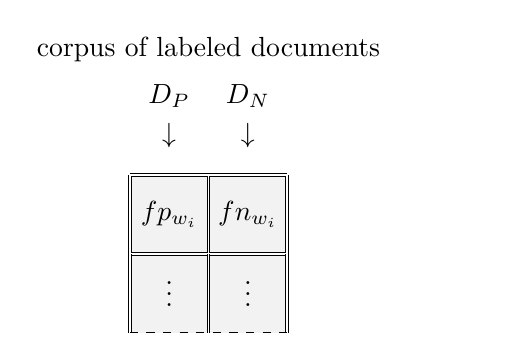
\begin{tikzpicture}
	\draw[step=1cm, opacity=0] (0,0) grid (4.5,0);
	\fill[black!5!white] (0,0) rectangle (2,2);
	\draw[step=1cm, double] (0,1) grid (2,2);
	\draw[step=1cm, double] (0,0) -- (0,1);
	\draw[step=1cm, double] (1,0) -- (1,1);
	\draw[step=1cm, double] (2,0) -- (2,1);
	\draw[step=1cm, dashed] (0,0) -- (2,0);
	%\node (p1) at (-0.5,1.5) {$\rightarrow$};
	%\node[left=-0.15cm of p1] {word $w_i$};
	\node at (1.0,3.6) {corpus of labeled documents};
	\node at (0.5,2.5) {$\downarrow$};
	\node at (1.5,2.5) {$\downarrow$};
	\node at (0.5,3) {$\mathbb{D}_\mathbb{P}$};
	\node at (1.5,3) {$\mathbb{D}_\mathbb{N}$};
	\node at (0.5,1.5) {$fp_{w_i}$};
	\node at (1.5,1.5) {$fn_{w_i}$};
	\node at (0.5,0.6) {$\vdots$};
	\node at (1.5,0.6) {$\vdots$};
\end{tikzpicture}
\caption[The frequency matrix of CopeOpi vectors]{The frequency matrix of CopeOpi vectors.\\
In the frequency matrix of CopeOpi vectors,
each row represents a unique word $w_i$ and
the $n$ columns represent $n$ corpora of labeled documents $\mathbb{D}_{c_1},\mathbb{D}_{c_2},\dots,\mathbb{D}_{c_n}$.
The element ${fc_j}_{w_i}$ is the frequency of word $w_i$
in corpus $\mathbb{D}_{c_j}$.
After $\mathbb{P}$ and $\mathbb{N}$ are grouped,
the two columns represent two corpora of labeled documents $\mathbb{D}_\mathbb{P}$ and $\mathbb{D}_\mathbb{N}$.
The elements $fp_{w_i}$ and $fn_{w_i}$ are the frequencies of word $w_i$ 
in corpus $\mathbb{D}_\mathbb{P}$ and in corpus $\mathbb{D}_\mathbb{N}$.}
\end{figure}
~\newline
~\newline
\clearpage
\partopic{One-versus-Rest\footnote{Also known as one-versus-all (OVA), one-against-rest (OAR), one-against-all (OAA).} Strategy (OVR)}
\par In an $n$-class text classification problem, we require $n$ augmented CopeOpi scores,
where each augmented CopeOpi score is computed to discriminate between one of the classes and the rest of the classes.
\begin{scheme}{CopeOpi Vectors (One-versus-Rest)}{}
Given $n$ corpora of labeled documents $\mathbb{D} = \{ \mathbb{D}_{c_1},\mathbb{D}_{c_2},\dots,\mathbb{D}_{c_n} \}$,
and the corresponding classes $\mathbb{C} = \{ c_1,c_2,\dots,c_n \}$.
\begin{itemize}
\item $\mathbb{D}_{c_i} = \{ \langle d,c \rangle \where \text{$d$ is a document labeled as class $c=c_i$} \}$
	\begin{itemize}
	\item the vocabulary $\mathbb{V}_{c_i}$ is a set of unique words in $\mathbb{D}_{c_i}$
	\end{itemize}
\end{itemize}
For each word $w_i \in \cup_{c \in \mathbb{C}} \mathbb{V}_{c}$,
we can compute its CopeOpi vector $\overrightarrow{\mathcal{COP}}_{w_i}$ by one-versus-rest strategy.
\tcbline
For each class $c_j \in \mathbb{C}$, we can construct two opposite sets,
\begin{itemize}
\item the positive set $\mathbb{P}^{c_j}_{w_i} = \{ c_j \}$
	\begin{itemize}
	\item the positive corpus ${\mathbb{D}_\mathbb{P}}^{c_j}_{w_i} = \{ \mathbb{D}_{c_j} \}$
	\item the positive vocabulary ${\mathbb{V}_\mathbb{P}}^{c_j}_{w_i} = \mathbb{V}_{c_j}$
	\end{itemize}
\item the negative set $\mathbb{N}^{c_j}_{w_i} = \mathbb{C} \setminus \{ c_j \}$
	\begin{itemize}
	\item the negative corpus ${\mathbb{D}_\mathbb{N}}^{c_j}_{w_i} = \mathbb{D} \setminus \{ \mathbb{D}_{c_j} \}$
	\item the negative vocabulary ${\mathbb{V}_\mathbb{N}}^{c_j}_{w_i} = \cup_{c \in \mathbb{N}^{c_j}_{w_i}} \mathbb{V}_{c}$
	\end{itemize}
\end{itemize}
and compute the augmented CopeOpi score $\mathcal{COP}^{c_j}_{w_i}$
of word $w_i$ with respect to class $c_j$ based on these two opposite sets.
\begin{equation*}
\begin{gathered}
	\mathcal{P}^{c_j}_{w_i} = \dfrac{
		fp^{c_j}_{w_i} \divby \sum_{w \in {\mathbb{V}_\mathbb{P}}^{c_j}_{w_i}} fp^{c_j}_w
	}{
		fp^{c_j}_{w_i} \divby \sum_{w \in {\mathbb{V}_\mathbb{P}}^{c_j}_{w_i}} fp^{c_j}_w +
		fn^{c_j}_{w_i} \divby \sum_{w \in {\mathbb{V}_\mathbb{N}}^{c_j}_{w_i}} fn^{c_j}_w
	}
\\[\eqlineskip]
	\mathcal{N}^{c_j}_{w_i} = \dfrac{
		fn^{c_j}_{w_i} \divby \sum_{w \in {\mathbb{V}_\mathbb{N}}^{c_j}_{w_i}} fn^{c_j}_w
	}{
		fp^{c_j}_{w_i} \divby \sum_{w \in {\mathbb{V}_\mathbb{P}}^{c_j}_{w_i}} fp^{c_j}_w +
		fn^{c_j}_{w_i} \divby \sum_{w \in {\mathbb{V}_\mathbb{N}}^{c_j}_{w_i}} fn^{c_j}_w
	}
\\[\eqlineskip]
	\mathcal{COP}^{c_j}_{w_i} = \mathcal{P}^{c_j}_{w_i} - \mathcal{N}^{c_j}_{w_i}
\end{gathered}
\end{equation*}
where $\mathcal{P}^{c_j}_{w_i}$ and $\mathcal{N}^{c_j}_{w_i}$ are the normalized probabilities of
word $w_i$ being in class $\mathbb{P}^{c_j}_{w_i}$ and being in class $\mathbb{N}^{c_j}_{w_i}$;
$fp^{c_j}_{w_i}$ and $fn^{c_j}_{w_i}$ are the frequencies of 
word $w_i$ in corpus ${\mathbb{D}_\mathbb{P}}^{c_j}_{w_i}$ and in corpus ${\mathbb{D}_\mathbb{N}}^{c_j}_{w_i}$;
the CopeOpi score $\mathcal{COP}^{c_j}_{w_i}$ of
word $w_i$ with respect to class $c_j$ is defined as the difference of the two opposite normalized probabilities, ranged from
$+1$(being in class $\mathbb{P}^{c_j}_{w_i}$) to $-1$(being in class $\mathbb{N}^{c_j}_{w_i}$).
\vspace{1.3\baselineskip}
\tcbline
The CopeOpi vector $\overrightarrow{\mathcal{COP}}_{w_i}$ of word $w_i$ is composed of these $n$ augmented CopeOpi scores.
~\newline
\begin{equation*}
\overrightarrow{\mathcal{COP}}_{w_i} = (\mathcal{COP}^{c_1}_{w_i},\mathcal{COP}^{c_2}_{w_i},\dots,\mathcal{COP}^{c_n}_{w_i})
\end{equation*}
\end{scheme}
\partopic{One-versus-One\footnote{Also known as one-against-one (OAO).} Strategy (OVO)}
\par In an $n$-class text classification problem, we require $\frac{1}{2}n(n-1)$ augmented CopeOpi scores,
where each augmented CopeOpi score is computed to discriminate between a pair of classes.
\begin{scheme}{CopeOpi Vectors (One-versus-One)}{}
Given $n$ corpora of labeled documents $\mathbb{D} = \{ \mathbb{D}_{c_1},\mathbb{D}_{c_2},\dots,\mathbb{D}_{c_n} \}$,
and the corresponding classes $\mathbb{C} = \{ c_1,c_2,\dots,c_n \}$.
\begin{itemize}
\item $\mathbb{D}_{c_i} = \{ \langle d,c \rangle \where \text{$d$ is a document labeled as class $c=c_i$} \}$
	\begin{itemize}
	\item the vocabulary $\mathbb{V}_{c_i}$ is a set of unique words in $\mathbb{D}_{c_i}$
	\end{itemize}
\end{itemize}
For each word $w_i \in \cup_{c \in \mathbb{C}} \mathbb{V}_{c}$,
we can compute its CopeOpi vector $\overrightarrow{\mathcal{COP}}_{w_i}$ by one-versus-one strategy.
\tcbline
For each class-pair $c_j,c_k \in \mathbb{C}$, $1 \leq j < k \leq n$, we can construct two opposite sets,
\begin{itemize}
\item the positive set $\mathbb{P}^{c_j,c_k}_{w_i} = \{ c_j \}$
	\begin{itemize}
	\item the positive corpus ${\mathbb{D}_\mathbb{P}}^{c_j,c_k}_{w_i} = \{ \mathbb{D}_{c_j} \}$
	\item the positive vocabulary ${\mathbb{V}_\mathbb{P}}^{c_j,c_k}_{w_i} = \mathbb{V}_{c_j}$
	\end{itemize}
\item the negative set $\mathbb{N}^{c_j,c_k}_{w_i} = \{ c_k \}$
	\begin{itemize}
	\item the negative corpus ${\mathbb{D}_\mathbb{N}}^{c_j,c_k}_{w_i} = \{ \mathbb{D}_{c_k} \}$
	\item the negative vocabulary ${\mathbb{V}_\mathbb{N}}^{c_j,c_k}_{w_i} = \mathbb{V}_{c_k}$
	\end{itemize}
\end{itemize}
and compute the augmented CopeOpi score $\mathcal{COP}^{c_j,c_k}_{w_i}$
of word $w_i$ with respect to class-pair $c_j,c_k$ based on these two opposite sets.

\begin{equation*}
\begin{gathered}
	\mathcal{P}^{c_j,c_k}_{w_i} = \dfrac{
		fp^{c_j,c_k}_{w_i} \divby \sum_{w \in {\mathbb{V}_\mathbb{P}}^{c_j,c_k}_{w_i}} fp^{c_j,c_k}_w
	}{
		fp^{c_j,c_k}_{w_i} \divby \sum_{w \in {\mathbb{V}_\mathbb{P}}^{c_j,c_k}_{w_i}} fp^{c_j,c_k}_w +
		fn^{c_j,c_k}_{w_i} \divby \sum_{w \in {\mathbb{V}_\mathbb{N}}^{c_j,c_k}_{w_i}} fn^{c_j,c_k}_w
	}
\\[\eqlineskip]
	\mathcal{N}^{c_j,c_k}_{w_i} = \dfrac{
		fn^{c_j,c_k}_{w_i} \divby \sum_{w \in {\mathbb{V}_\mathbb{N}}^{c_j,c_k}_{w_i}} fn^{c_j,c_k}_w
	}{
		fp^{c_j,c_k}_{w_i} \divby \sum_{w \in {\mathbb{V}_\mathbb{P}}^{c_j,c_k}_{w_i}} fp^{c_j,c_k}_w +
		fn^{c_j,c_k}_{w_i} \divby \sum_{w \in {\mathbb{V}_\mathbb{N}}^{c_j,c_k}_{w_i}} fn^{c_j,c_k}_w
	}
\\[\eqlineskip]
	\mathcal{COP}^{c_j,c_k}_{w_i} = \mathcal{P}^{c_j,c_k}_{w_i} - \mathcal{N}^{c_j,c_k}_{w_i}
\end{gathered}
\end{equation*}
where $\mathcal{P}^{c_j,c_k}_{w_i}$ and $\mathcal{N}^{c_j,c_k}_{w_i}$ are the normalized probabilities of
word $w_i$ being in class $\mathbb{P}^{c_j,c_k}_{w_i}$ and being in class $\mathbb{N}^{c_j,c_k}_{w_i}$;
$fp^{c_j,c_k}_{w_i}$ and $fn^{c_j,c_k}_{w_i}$ are the frequencies of 
word $w_i$ in corpus ${\mathbb{D}_\mathbb{P}}^{c_j,c_k}_{w_i}$ and in corpus ${\mathbb{D}_\mathbb{N}}^{c_j,c_k}_{w_i}$;
the CopeOpi score $\mathcal{COP}^{c_j,c_k}_{w_i}$ of
word $w_i$ with respect to class-pair $c_j,c_k$ is defined as the difference of the two opposite normalized probabilities, ranged from
$+1$(being in class $\mathbb{P}^{c_j,c_k}_{w_i}$) to $-1$(being in class $\mathbb{N}^{c_j,c_k}_{w_i}$).
\tcbline
The CopeOpi vector $\overrightarrow{\mathcal{COP}}_{w_i}$ of word $w_i$ is composed of these $\frac{1}{2}n(n-1)$ augmented CopeOpi scores.
\begin{equation*}
\overrightarrow{\mathcal{COP}}_{w_i} = (\mathcal{COP}^{c_1,c_2}_{w_i},\mathcal{COP}^{c_1,c_3}_{w_i},\dots,\mathcal{COP}^{c_{n-1},c_n}_{w_i})
\end{equation*}
\end{scheme}

\clearpage
\subsection{Customized CopeOpi Vectors}\label{sec:customized}
\par One-versus-rest strategy and one-versus-one strategy guide the basic way to construct CopeOpi vectors which can be applied to multiclass text classification.
\par However, in general, any subset of classes can be grouped as a positive set or a negative set. CopeOpi vectors can be customized based on different choices of subset-pairs.
~\newline
~\newline
\partopic{Subset-versus-Subset Strategy (SVS)}
\par In an $n$-class text classification problem, we can have at most $(2^n-1)^2$ augmented CopeOpi scores\footnote{We only eliminate the empty set cases, but not all subset-pairs can produce a discriminative augmented CopeOpi score.},
where each augmented CopeOpi score is computed to discriminate between a pair of subsets of classes.
\begin{scheme}{CopeOpi Vectors (Subset-versus-Subset)}{}
Given $n$ corpora of labeled documents $\mathbb{D} = \{ \mathbb{D}_{c_1},\mathbb{D}_{c_2},\dots,\mathbb{D}_{c_n} \}$,
and the corresponding classes $\mathbb{C} = \{ c_1,c_2,\dots,c_n \}$.
\begin{itemize}
\item $\mathbb{D}_{c_i} = \{ \langle d,c \rangle \where \text{$d$ is a document labeled as class $c=c_i$} \}$
	\begin{itemize}
	\item the vocabulary $\mathbb{V}_{c_i}$ is a set of unique words in $\mathbb{D}_{c_i}$
	\end{itemize}
\end{itemize}
For each word $w_i \in \cup_{c \in \mathbb{C}} \mathbb{V}_{c}$,
we can compute its CopeOpi vector $\overrightarrow{\mathcal{COP}}_{w_i}$ by subset-versus-subset strategy.
\tcbline
For any subset-pair $\mathbb{J},\mathbb{K} \subseteq \mathbb{C}$ where $\mathbb{J},\mathbb{K} \neq \varnothing$, can construct two opposite sets,
\begin{itemize}
\item the positive set $\mathbb{P}^{\mathbb{J},\mathbb{K}}_{w_i} = \mathbb{J}$
	\begin{itemize}
	\item the positive corpus ${\mathbb{D}_\mathbb{P}}^{\mathbb{J},\mathbb{K}}_{w_i} = \{ \mathbb{D}_{c} \where c \in \mathbb{J} \}$
	\item the positive vocabulary ${\mathbb{V}_\mathbb{P}}^{\mathbb{J},\mathbb{K}}_{w_i} = \cup_{c \in \mathbb{J}} \mathbb{V}_{c}$
	\end{itemize}
\item the positive set $\mathbb{N}^{\mathbb{J},\mathbb{K}}_{w_i} = \mathbb{K}$
	\begin{itemize}
	\item the positive corpus ${\mathbb{D}_\mathbb{N}}^{\mathbb{J},\mathbb{K}}_{w_i} = \{ \mathbb{D}_{c} \where c \in \mathbb{K} \}$
	\item the positive vocabulary ${\mathbb{V}_\mathbb{N}}^{\mathbb{J},\mathbb{K}}_{w_i} = \cup_{c \in \mathbb{K}} \mathbb{V}_{c}$
	\end{itemize}
\end{itemize}
and compute the augmented CopeOpi score $\mathcal{COP}^{\mathbb{J},\mathbb{K}}_{w_i}$
of word $w_i$ with respect to subset-pair $\mathbb{J},\mathbb{K}$ based on these two opposite sets.
\begin{equation*}
\begin{gathered}
	\mathcal{P}^{\mathbb{J},\mathbb{K}}_{w_i} = \dfrac{
		fp^{\mathbb{J},\mathbb{K}}_{w_i} \divby \sum_{w \in {\mathbb{V}_\mathbb{P}}^{\mathbb{J},\mathbb{K}}_{w_i}} fp^{\mathbb{J},\mathbb{K}}_w
	}{
		fp^{\mathbb{J},\mathbb{K}}_{w_i} \divby \sum_{w \in {\mathbb{V}_\mathbb{P}}^{\mathbb{J},\mathbb{K}}_{w_i}} fp^{\mathbb{J},\mathbb{K}}_w +
		fn^{\mathbb{J},\mathbb{K}}_{w_i} \divby \sum_{w \in {\mathbb{V}_\mathbb{N}}^{\mathbb{J},\mathbb{K}}_{w_i}} fn^{\mathbb{J},\mathbb{K}}_w
	}
\\[\eqlineskip]
	\mathcal{N}^{\mathbb{J},\mathbb{K}}_{w_i} = \dfrac{
		fn^{\mathbb{J},\mathbb{K}}_{w_i} \divby \sum_{w \in {\mathbb{V}_\mathbb{N}}^{\mathbb{J},\mathbb{K}}_{w_i}} fn^{\mathbb{J},\mathbb{K}}_w
	}{
		fp^{\mathbb{J},\mathbb{K}}_{w_i} \divby \sum_{w \in {\mathbb{V}_\mathbb{P}}^{\mathbb{J},\mathbb{K}}_{w_i}} fp^{\mathbb{J},\mathbb{K}}_w +
		fn^{\mathbb{J},\mathbb{K}}_{w_i} \divby \sum_{w \in {\mathbb{V}_\mathbb{N}}^{\mathbb{J},\mathbb{K}}_{w_i}} fn^{\mathbb{J},\mathbb{K}}_w
	}
\\[\eqlineskip]
	\mathcal{COP}^{\mathbb{J},\mathbb{K}}_{w_i} = \mathcal{P}^{\mathbb{J},\mathbb{K}}_{w_i} - \mathcal{N}^{\mathbb{J},\mathbb{K}}_{w_i}
\end{gathered}
\end{equation*}
where $\mathcal{P}^{\mathbb{J},\mathbb{K}}_{w_i}$ and $\mathcal{N}^{\mathbb{J},\mathbb{K}}_{w_i}$ are the normalized probabilities of
word $w_i$ being in class $\mathbb{P}^{\mathbb{J},\mathbb{K}}_{w_i}$ and being in class $\mathbb{N}^{\mathbb{J},\mathbb{K}}_{w_i}$;
$fp^{\mathbb{J},\mathbb{K}}_{w_i}$ and $fn^{\mathbb{J},\mathbb{K}}_{w_i}$ are the frequencies of 
word $w_i$ in corpus ${\mathbb{D}_\mathbb{P}}^{\mathbb{J},\mathbb{K}}_{w_i}$ and in corpus ${\mathbb{D}_\mathbb{N}}^{\mathbb{J},\mathbb{K}}_{w_i}$;
the CopeOpi score $\mathcal{COP}^{\mathbb{J},\mathbb{K}}_{w_i}$ of
word $w_i$ with respect to subset-pair $\mathbb{J},\mathbb{K}$ is defined as the difference of the two opposite normalized probabilities, ranged from
$+1$(being in class $\mathbb{P}^{\mathbb{J},\mathbb{K}}_{w_i}$) to $-1$(being in class $\mathbb{N}^{\mathbb{J},\mathbb{K}}_{w_i}$).
\tcbline
The CopeOpi vector $\overrightarrow{\mathcal{COP}}_{w_i}$ of word $w_i$ is composed of these at most $(2^n-1)^2$ augmented CopeOpi scores.
\begin{equation*}
\overrightarrow{\mathcal{COP}}_{w_i} = (\mathcal{COP}^{\mathbb{J}_1,\mathbb{K}_1}_{w_i},\mathcal{COP}^{\mathbb{J}_2,\mathbb{K}_2}_{w_i},\dots)
\end{equation*}
\end{scheme}